%!TEX root=../../main.tex

\chapter{Multiple Linear Regression}
\label{multipleLinearRegression}
\index{multiple linear regression|textbf}



Simple linear regression is useful when the main interest of a study is the association of a response variable with a single predictor or explanatory variable.  Scientific investigations are rarely that simple, however; in most settings more than one explanatory variable is likely to be associated with a response, and multiple linear regression can be important model in those situations.  The study of risk factors for cognitive decline in adults outlined in the next section is one of those situations.

Section~\ref{introductionMultipleLinearRegression} discusses the concept
of confounding, when the apparent association between a response and a
primary predictor might be distorted when a third variable associated
with both the response and the predictor is ignored.  In the example
used, the response variable is a measure of cognitive decline
(\var{RFFT} in the PREVEND data), the primary predictor of interest is
the use of a drug to lower cholesterol and the possible confounder is
age. 

Sections~\ref{simpleVsMultipleRegression} shows how multiple regression
can be used to estimate the association between RFFT and statin use,
after adjusting for age.  Adjusting for one or more possible confounders
is not the only application of multiple regression, but it is one of the
more important.   The model used is a simple model with two predictors
but it illustrates many of the important ideas in multiple regression;
it is a good way to start the study of more complicated models and other
applications.

Section~\ref{Evaluating the fit of a multiple regression model} continues with a model with two predictors, showing methods for evaluating the quality of the fit of the model. Section~\ref{generalMultipleRegression} then outlines the general ideas of multiple regression.  Additional applications of multiple regression are illustrated in the last three sections of the chapter.

\section{Introduction to multiple linear regression}
\label{introductionMultipleLinearRegression}

Statins are a class of drugs that widely used to lower cholesterol. Cholesterol is measured using both low density lipoprotein (LDL) and high density lipoprotein (HDL).  Total cholesterol is the sum of LDL and HDL.  Research has suggested that an adult with elevated LDL may be at risk for adverse cardiovascular events, such as a heart attach or a stroke.  In 2013, an expert panel commissioned by the American College of Cardiology and the American Heart Association recommended that statin therapy be considered in an individual with any form of atherosclerotic cardiovascular disease (arteries that are becoming clogged with plaque), with primary LDL cholesterol levels $\ge$ 190 mg/dL, with type 2 diabetes, with age 40 - 75 and LDL between 70 and 189 mg/dL, or an individual without diabetes but age 40 - 75 and with a predicted probability of future clogged arteries of at least 0.075\footnote{Circulation. 2014;129:S1-S45. DOI: 10.1161/01.cir.0000437738.63853.7a}.

Some health policy analysts have estimated that if the new guidelines were to be followed strictly, almost half of Americans ages 40 to 75 and nearly all men over 60 would be prescribed a statin. In addition to cardiovascular disease, however, older adults are also at risk for cognitive decline and, in severe cases, dementia, and some physicians have raised the question of whether treatment with a statin might be associated with an increased risk of cognitive decline\footnote{Muldoon, Matthew F., et al. Randomized trial of the effects of simvastatin on cognitive functioning in hypercholesterolemic adults. The American journal of medicine 117.11 (2004): 823-829.}\footnote{King, Deborah S., et al. Cognitive impairment associated with atorvastatin and simvastatin. Pharmacotherapy: The Journal of Human Pharmacology and Drug Therapy 23.12 (2003): 1663-1667.}.  The study by Joosten, et al.\footnote{Joosten H, Visser ST, van Eersel ME, Gansevoort RT, Bilo HJG, et al. (2014) Statin Use and Cognitive Function: Population-Based Observational Study with Long-Term Follow- Up. PLoS ONE 9(12): e115755. doi:10.1371/ journal.pone.0115755} examined the association of statin use and other variables with cognitive ability in an observational cohort of 4095 participants from the Netherlands who were part of the larger PREVEND introduced in Section~\ref{examiningScatterPlots}.  This section presents an analysis based on a random sample of 500 participants from the cohort using one measure of cognitive ability and a few important predictors.  The dataset \data{statins.samp} used in this analysis is contained and is documented in the package \it{OIBioStat}.

\begin{comment}
\textit{The pair of footnotes for muldoon and king appear as 23 instead of 2,3.  usepackage[multiple]{footnotemisc} should solve this but produces an error  -- clash of options. Not sure what it is clashing with.}  Not resolved yet.

\end{comment} 
 
Precise measurements of cognitive ability are difficult, perhaps even impossible.  Cognitive ability fluctuates mildly in elders from day to day and affects speech, reading, the ability to complete tasks and many other aspects of life.  Participants in the Joosten study were asked to complete the Ruff Figural Fluency Test (RFFT)\footnote{Ruff, Ronald M., Rudolph H. Light, and Randall W. Evans. "The Ruff Figural Fluency Test: a normative study with adults." Developmental Neuropsychology 3.1 (1987): 37-51.}, in which scores range from 0 (worst) to 175 (best).  In the test, participants complete as many designs as possible in a time limit, using a pattern of dots on a page.  The test is thought to be a measure of executive function.  Even with a reasonable measurement of cognitive function, the investigators anticipated an issue in the analysis: statins are used more often in older than in younger adults, and older adults suffer a natural cognitive decline.  Age is a potential \term{confounder} in this setting -- if age is ignored in the analysis, the tendency for older people to be treated with statins and to suffer cognitive decline might make it appear that cognitive decline is more common among individuals prescribed statins, simply because those prescribed statins are older than those not prescribed statins.

In the dataset \data{statins.samp}, the scatterplot of \var{Age} vs \var{RFFT} in Figure~\ref{statinAgeRFFTConfounderPlot} shows why \var{Age} is a potential confounder for the association between statin use and RFFT.  The points in the figure are appear in two colors, blue if a participant is not using statins, and red if he or she is.  First, it is clear that statin use increases with age, so age and statin use are associated.  Second, ignoring the colors, it is also clear that age is associated with lower RFFT scores, since the point cloud drifts down and to the right.  But a close inspection of the plot suggests that for ages in relatively small ranges (e.g., age 50 - 60), statin use may not be strongly associated with RFFT score -- there are approximately as many red dots with low RFFT scores as with high RFFT scores.  In subsets of participants with approximately the same age, statin use may not associated with RFFT. Multiple regression provides a way to estimate the association of statin use with RFFT after adjusting for age.  Essentially, it provides an estimate of the association of statin use and RFFT within age groups.

\begin{figure}[h!]
	\centering
	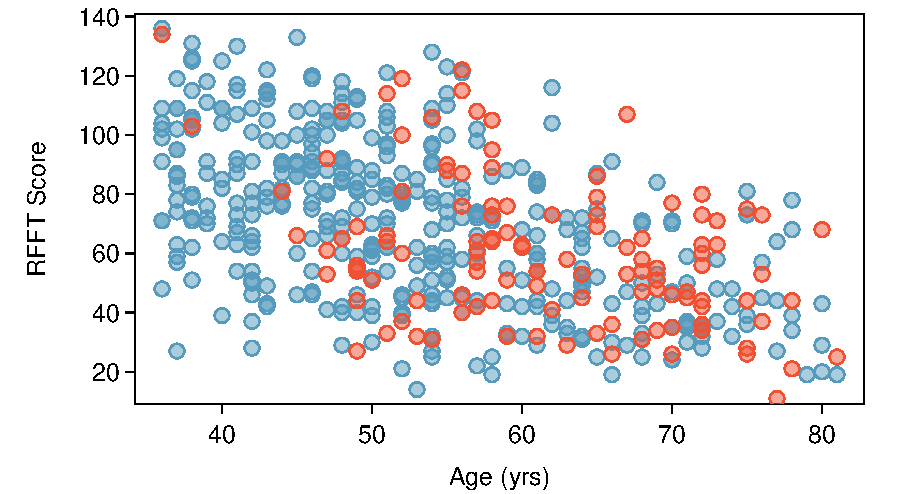
\includegraphics[width=0.8\textwidth]
	{ch_multiple_linear_regression_oi_biostat/figures/statinAgeRFFTConfounderPlot/statinAgeRFFTConfounderPlot}
	\caption{A scatterplot showing \var{age} vs. \var{RFFT}. Points for participants using statins are in red; points for participants not using statins are in black.}
	\label{statinAgeRFFTConfounderPlot}
\end{figure}

\section{Simple vs. multiple regression}
\label{simpleVsMultipleRegression}

The dataset \data{statin.samp} contains observations on a random sample of 500 participants from the PREVEND study, and was introduced in Section~\ref{examiningScatterPlots}.  The variable \var{Statin} is coded 1 if the participant was using a statin at the time of the study, and 0 if not.  

Figure~\ref{statinRFFTPlots} shows on the left a histogram of the RFFT scores, and on the right a scatterplot of categorical predictor \var{Statin} vs the response variable \var{RFFT}.  The RFFT scores are approximately  symmetrically distributed with no extreme outliers, and the negative slope of the least squares regression line in the scatterplot indicates a possible negative association between RFFT cores and statin use.

\begin{figure}[ht]
	\centering
	\subfigure[]{
		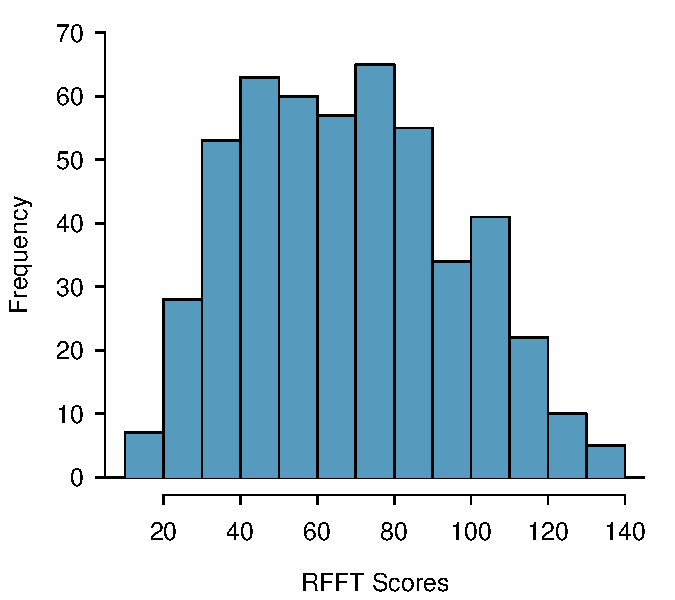
\includegraphics[width=0.46\textwidth]
		{ch_multiple_linear_regression_oi_biostat/figures/statinRFFTPlots/RFFTHist}
		\label{RFFTHist}
	}
	\subfigure[]{
		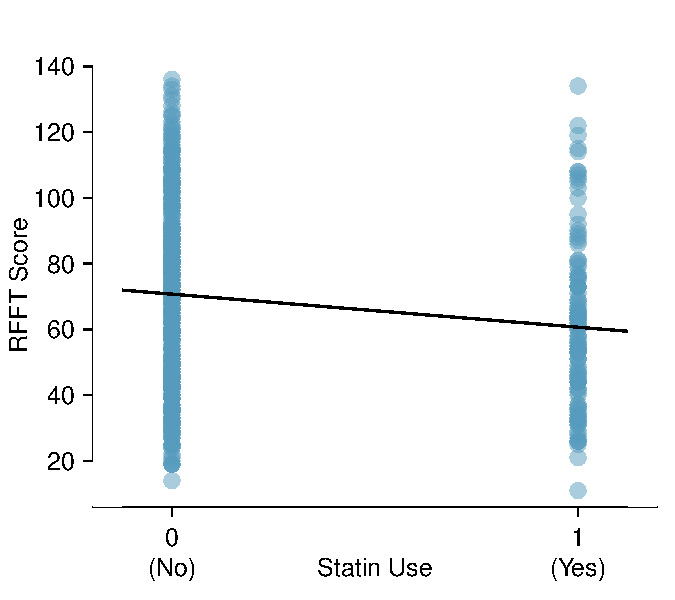
\includegraphics[width=0.46\textwidth]
		{ch_multiple_linear_regression_oi_biostat/figures/statinRFFTPlots/statinRFFTDotPlot}
		\label{statinRFFTDotPlot}
	}
	\caption{\subref{RFFTHist} Histogram of RFFT Scores. \subref{statinRFFTDotPlot} scatterplot of statin use vs RFFT score.}
	\label{statinRFFTPlots}
\end{figure}


A simple linear regression model
\[
   E(\text{RFFT}) = \beta_0 + \beta_{\text{Statin}}\text{Statin}
   \label{RFFTStatinModel}
\]
can be used initially to examine the association between the categorical variable \var{Statin} use and score on the RFFT scale.  As noted in Chapter 6, this form of the regression model is equivalent to 
\[
   \text{RFFT} = \beta_0 + \beta_{\text{Statin}}\text{Statin} + \varepsilon
\]

Table~\ref{RFFTStatinRegression} gives the parameters of the least squares line in Figure~\ref{statinRFFTDotPlot}.

Here is the output from \textsf{R}:

\begin{table}[ht]
\centering
\begin{tabular}{rrrrr}
  \hline
 & Estimate & Std. Error & t value & Pr($>$$|$t$|$) \\ 
  \hline
(Intercept) & 70.7143 & 1.3808 & 51.21 & 0.0000 \\ 
  Statin & -10.0534 & 2.8792 & -3.49 & 0.0005 \\ 
   \hline
\end{tabular}
\caption{Parameter estimates for the least squares line of RFFT vs statin use in the PREVEND data.}
\label{RFFTStatinRegression}
\end{table} 
%xtable(summary(lm(RFFT ~ Statin, data=statins.samp)))
% latex table generated in R 3.2.3 by xtable 1.8-0 package
% Wed Nov  2 14:30:27 2016
The $R^2$ for this model is 0.0239.
 
Even though the use of a statin drug explains only 2.4\% of the variability in the RFFT scores, the table does show that statin use is significantly associated with RFFT score. Statin users (those with value 1 in \var{statin}) score approximately 10 points lower on average in the RFFT test.  But the result may be confounded by age, as discussed earlier.   The boxplot in Figure~\ref{statinAgeBoxPlot} confirms that statin users tend to be older, and the scatterplot in Figure~\ref{statinAgeRFFTConfounderPlot} showed a clear linear trend in declining RFFT scores for older adults, regardless of statin use.  In fact, the regression output shown in Table~\ref{RFFTAgeRegression} shows that age has a strongly significant association with RFFT score.
 
 \begin{figure}[h!]
 	\centering
 	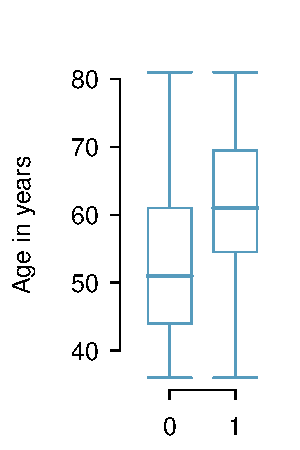
\includegraphics[width=0.4\textwidth]
	{ch_multiple_linear_regression_oi_biostat/figures/statinAgeBoxPlot/statinAgeBoxPlot.pdf}
 	\caption{Boxplot of age by statin use; 0 = participant not using statins, 1 = using statins. PREVEND data.}
	\label{statinAgeBoxPlot}
 \end{figure}
 
% latex table generated in R 3.4.2 by xtable 1.8-2 package
% Fri Dec 29 10:00:07 2017
% p-value edited
\begin{table}[ht]
\centering
\begin{tabular}{rrrrr}
  \hline
 & Estimate & Std. Error & t value & Pr($>$$|$t$|$) \\ 
  \hline
(Intercept) & 137.5497 & 5.0161 & 27.42 & < 0.001 \\ 
  Age & -1.2614 & 0.0895 & -14.09 & < 0.001 \\ 
   \hline
\end{tabular}
\caption{R output from the regression of the 
       response variab RFFT with predictor Age} 
\label{RFFTAgeRegression}
\end{table}


The model for multiple linear regression with two predictors is a straightforward extension of simple regression and can be used to adjust for confounders.  

In the PREVEND data, a model for RFFT that incorporates both statin use and age is
 \[
    E(\text{RFFT}) = \beta_0 + \beta_{\text{Statin}}\text{Statin} + \beta_{\text{Age}}\text{Age}.
	\label{RFFTStatinAgeEquation}
 \]
An investigator might use this model to examine the possible change in the association between \var{RFFT} and statin use when the confounder \var{Age} is included in the model.  In statistical terms, the association between \var{RFFT} and \var{Statin} is being estimated after adjusting for \var{Age}.

More generally, if $Y$ is a response variable and $X_1$ and $X_2$ are two predictors, a regression model with two variables has the form 
\[
Y = \beta_0 + \beta_1 X_1 + \beta_2 X_2 + \varepsilon,
\]
or, equivalently,
\[
E(Y) = \beta_0 + \beta_1 X_1 + \beta_2 X_2,
\]
since $\varepsilon$ is assumed to have mean 0.  Section~\ref{generalMultipleRegression} outlines the principles and assumptions behind the multiple regression model with two or more predictors and the method used to estimate the coefficients, but it is not difficult to fit these models in software.  Table~\ref{RFFTStatinAgeRegression} shows the estimated regression model for the association of the response variable \var{RFFT} with both statin use and age, using \textsl{R}.  
 
 \begin{table}[ht]
 \centering
 \begin{tabular}{rrrrr}
   \hline
  & Estimate & Std. Error & t value & Pr($>$$|$t$|$) \\ 
   \hline
 (Intercept) & 137.8822 & 5.1221 & 26.92 & 0.0000 \\ 
   Statin & 0.8509 & 2.5957 & 0.33 & 0.7432 \\ 
   Age & -1.2710 & 0.0943 & -13.48 & 0.0000 \\ 
    \hline
 \end{tabular}
 \caption{Parameter estimates in the multiple regression for RFFT vs statin use and age in the PREVEND data.}
 \label{RFFTStatinAgeRegression}
 \end{table}
 % xtable(summary(lm(RFFT ~ Statin + Age, data=statins.samp)))
 % latex table generated in R 3.3.1 by xtable 1.8-2 package
 % Fri Nov  4 10:01:01 2016
 

The information in Table~\ref{RFFTStatinAgeRegression} is used in much the same way that a table showing estimates in simple regression would be used.

\begin{itemize}
	
	\item The coefficients for \var{Statin} and \var{Age} can be used in a prediction.  The predicted RFFT score for a 67 year old using statins (\var{Statin} = 1) is 
	\[
	 \widehat{\text{RFFT}} = 137.822 + (0.8509)(1) - (1.2710)(67) = 53.5159.
	\]
The predicted RFFT for a 67 year old not using statins is
	\[
	 \widehat{\text{RFFT}} = 137.822 + (0.8509)(0) - (1.2710)(67) = 52.6650.
	\]
    The predicted RFFT score increases by 0.8509, the value of the \var{Statin} coefficient.  This is the most striking feature of the table -- in a model that includes \var{Age}, statin use seems to be associated with an increase in RFFT, rather than a decrease, as in the simple regression.

A simple calculation shows that this change in RFFT would have been the same for statin user vs non-user regardless of the value of \var{Age}, as long as the age is the same for the two participants. The coefficient for \var{Statin} is the change in predicted RFFT score for two individuals of the same age, but differing in whether they are taking statins.  In most cases, predictions are not calculated to so many significant digits, since the coefficients are only estimates.  This example uses the additional precision to illustrate the role of the coefficients.
	
	\item  Suppose neither of two participants was taking statins (\var{Statin} = 0), one 65 years old and the other 66.  The two predicted RFFT scores would be  55.207 and 53.936. The change in the predicted scores (-1.271) is the value of the coefficient for \var{Age}, because \var{Age} has changed by one year (one unit on the age scale).   A simple calculation shows that this predicted change would have been the same for two individuals 65 and 66 years old, both taking statins.  The coefficient for \var{Age} is the change in predicted RFFT score if age differs by one year and statin use is the same.
	
	\item Residuals in multiple regression are the differences between observed and predicted values for each case in the dataset, just as in simple regression.  In the sample of 500 cases used to estimate the regression model, there is a participant age 67, using statins, and whose RFFT score is 53.  The residual for that case would be $53 - 53.5150 = - 0.5159$.
	
 \item  The sign of the coefficients for the two predictors specifies the direction of change in the response RFFT when one of the predictors changes. Taking statins is associated with a small increase in RFFT score, while older age is associated with decreasing RFFT scores.
 
 \item  For each of the two coefficients, the $t$-statistic is the ratio of the estimated coefficient divided by its standard error.  Standard errors are more complicated to multiple regression than in simple regression, but they serve the same purpose.  They are an estimate of the standard deviation of the coefficient.  As in simple regression, the $t$-statistics can be used to test the two null hypotheses $H_0:\beta_{\text{Statin}} = 0$ or $H_0:\beta_{\text{Age}} = 0$ against two-sided alternatives.
  
  \item In a model with two predictors, the sampling distributions of the $t$-statistics for each of the parameters are $t$-distributions with $n - 2$ degrees of freedom, where $n$ is the number of cases used to estimate the regression. The last column in the table contains the two-sided $p$-values for these two hypothesis tests, just as in simple regression.  These $p$-values indicate that when using $\alpha = 0.05$ the association between statin use and RFFT score is not statistically significant, but the association between age and RFFT is significant.
  
  \item  The result of the analysis can be summarized with the statement, ``Although the use of statins appeared to be associated with lower RFFT scores when no adjustment has been made for possible confounders, statins are not significantly associated with RFFT score in a regression model that adjusts for age.  The association of age with RFFT is statistically significant; older participants had lower scores.''
  
  \item Just as in simple linear regression, the coefficient for the intercept must be interpreted with care.  In this model, the intercept gives the predicted RFFT for someone not using statins and of age 0, and is clearly meaningless.
  
  \item There is an important aspect of these data that should not be overlooked.  The data do not come from a study in which participants were followed as they aged, allowing for the measurement of changing RFFT in a participant over time. Such a study is called a longitudinal study.  This study was a cross-sectional study -- patient age, statin use and RFFT were recorded for all participants during a short time interval.  The results of the study support the conclusion that older patients tend to have lower RFFT scores, but cannot be used to conclude that scores decline with age in individuals.  Older patients come from an earlier birth cohort, and it is possible, for instance, that younger participants have more post-secondary school education or better health practices generally.  In other words, there may be a cohort effect.  This is an important point to be aware of, and is not at all evident in the Table~\ref{RFFTStatinAgeRegression}
  
 \end{itemize}
 
 
The results of the analysis shown in Table~\ref{RFFTStatinAgeRegression} provide an initial look at the association between RFFT score, statin use and age. There is, however, no information about either the quality of the fit or its potential value for predictions. The next section describes the residual plots that can be used to check some of the model assumptions and the use of $R^2$ to estimate how much of the variability in the response variable is explained by the model.

\section{Evaluating the fit of a multiple regression model}

\subsection{Using residuals to check model assumptions}

The assumptions behind multiple regression are essentially the same as the 4 assumptions listed in Section~\ref{examiningScatterplots}.  The assumption of linearity is extended to multiple regression by assuming that when only one predictor changes, it is linearly related to the change in the response variable.  Assumption 2 becomes the slightly more general assumption that the residuals have approximately constant variance, and Assumption 4 is simply that the residuals are approximately normally distributed. Assumption 3 that the observations on each case are independent does not change. 

Residual plots are useful in checking modeling assumptions in multiple
regression, perhaps even more so than in simple linear regression since
it is not possible to make a scatterplot of a response variable against
several simultaneous predictors.  It is possible to plot predicted
values vs residuals, since each case has one predicted value and one
residual. The patterns in these residual plots that might indicate lack
of fit are the same as in Figure~\ref{sampleLinesAndResPlots} from
Chapter~\ref{linRegrForTwoVar}. Just as in simple regression, normal
probability plots can be used to check the normality assumption of the
residuals.  The scatterplot of predicted values vs residuals from the
estimated model in Table~\ref{RFFTStatinAgeRegression} is in the left
panel of Figure~\ref{statinAgeResidNormPlot} and shows that the
residuals have slightly smaller variance for small predicted values of
RFFT, but that the variability of the residuals is otherwise
approximately constant.  The normal probability plot in the left panel
shows that the residuals from the model are reasonably normally
distributed, with departures from normality in the tails.


\begin{figure}[h!]
	\centering
	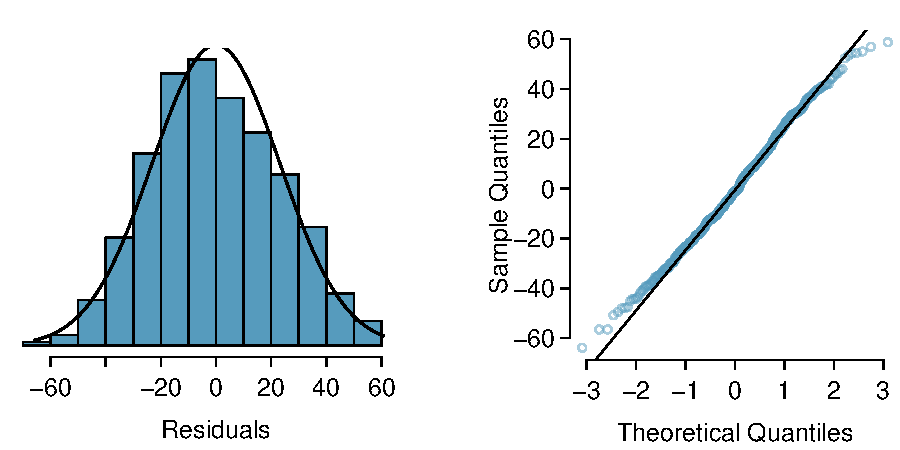
\includegraphics[width=0.8\textwidth]
	{ch_multiple_linear_regression_oi_biostat/figures/statinAgeResidNormPlot/statinAgeResidNormPlot.pdf}
	\caption{A histogram and normal probability plot of the residuals from the linear model for RFFT vs. statin use and age in the PREVEND data}
	\label{statinAgeResidNormPlot}
\end{figure}


Examining plots of residuals against each of the predictors can be useful with multiple regression, since they might show a nonlinear trend in an association with one of the variables that might be corrected with a transformation.  The scatterplot of residuals from the model in Table~\ref{RFFTStatinAgeRegression} vs Age shows no apparent nonlinear trends.  


\begin{figure}[h!]
	\centering
	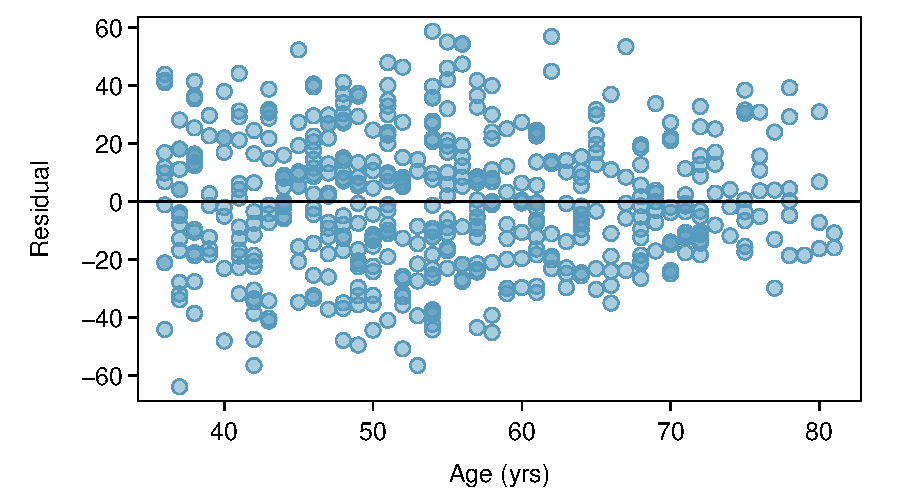
\includegraphics[width=0.8\textwidth]
	{ch_multiple_linear_regression_oi_biostat/figures/statinAgeResidPlot/statinAgeResidPlot.pdf}
	\caption{Age vs residuals in the model for RFFT vs statins and age in the PREVEND data.  The horizontal line is the least squares line for age vs the residuals.}
	\label{statinAgeResidPlot}
\end{figure}


\subsection{Using $R^2$ and adjusted $R^2$ with multiple regression}
\index{adjusted r squared@adjusted $R^2$ ($R_{adj}^2$)|(}


Section~\ref{RSquaredLinearRegression} provided two definitions of the statistic $R^2$ -- it is the square of the correlation coefficient $r$ between a response and the single predictor in simple linear regression, and it is equivalently the proportion of the variation in the response variable explained by the simple regression model.  In statistical terms, the second definition can be written as 
\begin{align*}
   R^2 &= \frac{\text{var}(y_i) - \text{var}(e_i)}
   {\text{var}(y_i)}\\
   &= 1 - \frac{\text{var}(e_i)}{\text{var}(y_i)},
   \label{RSquareDefinition}
\end{align*}
where $y_i$ and $e_i$ denote the response and residual values for the
i$th$ case.

The first definition cannot be used in multiple regression, since there is a correlation coefficient between each predictor and the response variable instead of a single correlation between one predictor and a response.  The second defintion, however, can be used for $R^2$ multiple regression, since there is a single set of residuals.

The equation for $R^2$ can be used to calculate it directly, but since $R^2$ is a standard part of the output from regression software it is rarely calculated by hand. In software output, $R^2$ usually labeled `multiple R-squared'. In the  model with response \var{RFFT} and predictors \var{Statin} and \var{Age} , $R^2 = 0.2852$.  The model explains almost 29\% of the variability in RFFT scores, a considerable improvement over the model with \var{Statin} alone.

Advanced courses in regression show that adding a variable to a regression model always increases the value of $R^2$.  Sometimes that increase is large and clearly important, as when \var{Age} is added to the model for RFFT scores.  Sometimes the increase is small, and may not be worth the added complexity of the model.  The statistic \term{adjusted R-squared} is often used in multiple regression to balance model predictive ability with complexity.

\begin{termBox}{\tBoxTitle{Adjusted $\mathbf{R^2}$ as a tool for model assessment}
The \termsub{adjusted $\mathbf{R^2}$}{adjusted r squared@adjusted $R^2$ ($R_{adj}^2$)} is computed as
\begin{align*}
R_{adj}^{2} = 1-\frac{\text{Var}(e_i) / (n-p-1)}{\text{Var}(y_i) / (n-1)}
	= 1-\frac{\text{Var}(e_i)}{\text{Var}(y_i)} \times
    \frac{n-1}{n-p-1},
\end{align*}
where $n$ is the number of cases used to fit the model and $p$ is the number of predictor variables in the model.}
\end{termBox}

Since $p = 1$ in simple linear regression, the $R^2$ and adjusted $R^2$ have the same value when there is only a single predictor.

The adjusted $R^2$ is also routinely provided in software.  The value of the adjusted $R^2$ in the model with both \var{Statin} and \var{Age} is 0.2823 -- the additional predictor \var{Age} adds only moderate complexity while increasing the strength of model considerably.

%DH: \textit{guided practice to calculate adjusted R-squared by hand could be inserted  here}

Multiple regression is widely used in many types of applications, from medical and biological research to the social sciences. Entire books and advanced courses devoted to its study.  The next section outlines the general framework for multiple regression and provides the material needed for more complex models.
 
 \section{The general multiple linear regression model}
 \label{generalMultipleRegression}
 
Sections~\ref{introductionMultipleLinearRegression} and \ref{simpleVsMultipleRegression} introduced multiple regression with two predictors as a technique to estimate an association of primary interest in the presence of confounding.  Multiple regression has many more uses -- it can be used to build a model for prediction responses, for learning which subset of variables in a set of potential predictors are associated with the response, and as a unified approach to ANOVA.

This section provides a compact summary of the multiple regression model and has more mathematical detail than most other sections.  Using an extended analysis of the PREVEND data, Section~\ref{reanalyzingStatinDataSet} illustrates the ideas outlined here and in the next section.  It is best to read this and the next section once for the main ideas, then refer back to them when reading the subsequent section.
 
 
\subsection{Model parameters and least squares estimation}
 
For multiple regression, the data consist of a response variable $Y$ and $p$ potential predictors or explanatory variables $X_1, X_2,\ldots, X_p$.   Instead of the simple regression model 
 $${Y} = \beta_{0} + \beta_{1}X + {\varepsilon},$$
 multiple regression has the form
 $${Y} = \beta_{0} +
     \beta_{1}X_{1} + \beta_{2}X_{2} + \beta_{3}X_{3} + \dots +
     \beta_{p}X_{p} + \varepsilon,$$
or equivalently
 $$E(Y) = \beta_{0} + 
     \beta_{1}X_{1} + \beta_{2}X_{2} + \beta_{3}X_{3} + \dots +
     \beta_{p}X_{p},
	 \label{multipleRegressionModel}
	 $$ 
since the normally distributed error term $\varepsilon$ is assumed to have mean 0. Each predictor $x_i$ has an associated coefficient $\beta_i$.  In simple regression, the slope coefficient $\beta$ captures the change in the response variable $Y$ associated with a 1 unit  change in the predictor $X$.  In multiple regression, the coefficient $\beta_j$ of a predictor $X_j$ denotes the change in the response variable $Y$ associated with a one unit change in $X_j$ when none of the other predictors change.  So each $\beta$ coefficient in multiple regression plays the role of a slope, as long as the other predictors are not changing.

In words, multiple regression is the model for the mean of the response $Y$ in a population where the that mean is not constant but depends on the values of the predictors.  In a setting with two binary predictors such as statin use and sex (coded as \var{gender} in \data{statins}\footnote{Until recently, it was common practice to use \var{gender} to denote biological sex. Gender is different than biological sex, but this text uses the original names in published datasets}), the predictors would partition the population into 4 subgroups (statin use yes/no, female/male), and the predicted values from the model would be estimates of the mean in each of the four groups.

\begin{exercise}
The table below shows an estimated regression model for \var{RFFT} with predictors \var{Statin} and \var{Gender}, where \var{Gender} is coded 0 for males and 1 for females.  Based on the model, what are the estimated mean RFFT scores for the four groups defined by statin use and gender? 
	% xtable(summary(lm(RFFT ~ Statin + Gender, data=statins.samp)))
	% latex table generated in R 3.3.1 by xtable 1.8-2 package
	% Mon Dec  5 09:40:50 2016
	\begin{table}[ht]
	\centering
	\begin{tabular}{rrrrr}
	  \hline
	 & Estimate & Std. Error & t value & Pr($>$$|$t$|$) \\ 
	  \hline
	(Intercept) & 70.4068 & 1.8477 & 38.11 & 0.0000 \\ 
	  Statin & -9.9700 & 2.9011 & -3.44 & 0.0006 \\ 
	  Gender & 0.6133 & 2.4461 & 0.25 & 0.8021 \\ 
	   \hline
	\end{tabular}
	\end{table}
\end{exercise}

Datasets for multiple regression have $n$ cases, usually indexed algebraically by $i$, where $i$ takes on values from 1 (first case in the dataset) to $n$ (last case).  The dataset \data{statins.samp} contains $n = 500$ observations.  Algebraic representations of the data must denote both the case number and the predictor in the set of $p$ predictors. The variable $X_{ij}$ denotes predictor $X_j$ for case $i$ in the dataset.  The response for case $i$ is simply $Y_i$. The dataset \data{statins.samp} has many possible predictors, some of which are examined later in this chapter.  The analysis in Section~\ref{simpleVsMultipleRegression} used $p=2$ predictors, \var{Statin} and \var{Age}.

Just as in Chapter~\ref{probability}, upper case letters are used when thinking of data as a set of random observations subject to sampling from a population, and lower case letters are used for observed values.  With this notation, row $i$ of dataset with $n$ cases and $p$ predictors can be written as $(y_i, x_{i1}, x_{i2}, \ldots, x_{ip})$.

Estimates of the coefficients $\beta_1,\beta_2,\ldots, \beta_p$ are obtained using the principle of least squares.  For any given set of estimates $b_1, b_2,\ldots,b_p$ and predictors $x_{i1},x_{i2},\ldots,x_{ip}$, predicted values of the response can be calculated using
\[
   \hat{y}_i = b_0 + b_1 x_{i1} + b_2 x_{i2} +\cdots b_p x_{ip},
\]
and the residual from the prediction is the difference between the observed value $y_i$ and predicted value $\hat{y_i}$, or $e_i = y_i - \hat{y}_i$.  The least squares estimate of the model is the set of estimated coefficients $b_0, b_1, \ldots b_p$ that minimizes $e_1^2 + e_2^2 + \cdots e_n^2$.  This approach is identical in concept to the use of least squares in simple linear regression.

Explicit formulas for the estimates involve advanced matrix theory, but are rarely used in practice.  Instead, estimates are calculated using software such as as \textsf{R}, Stata or Minitab are used.

\subsection{Hypothesis tests and confidence intervals with multiple regression}

\textbf{Using $t$-tests for individual coefficients}

When a coefficient of a predictor in the multiple regression~\ref{multipleRegressionModel} model is 0, the predicted value of the response does not change when the predictor changes.  In statistical terms, that predictor is not associated with the response variable.  Because of the inherent variability in observed data, an estimated coefficient will almost never be 0 even when the model coefficient is.  But the result from a regression can be used to test the null hypothesis that the coefficient is 0 by examining the ratio of the estimated coefficient to its standard error.  When the assumptions of a multiple regression hold, at least approximately, this ratio has a $t$-distribution with $n - (p + 1) =n - p - 1$ degrees of freedom when the model coefficient is 0. The formula for the degrees of freedom follows a general rule that appears throughout statistics -- the degrees of freedom for an estimated model is the number of cases in the dataset minus the number of estimated parameters.  There are $p + 1$ parameters in the multiple regression model, one for each of the $p$ predictors and one for the intercept.

\begin{termBox}{\tBoxTitle{Sampling distributions of estimated coefficients}
Suppose 
\[
\hat{y} = b_0 + b_1 x_{i} + b_2 x_{i} +\cdots b_p x_{i}
\]
is an estimated multiple regression model from a dataset with $n$ observations on response and predictor variables, and let $b_k$ be one of the estimated coefficients.  Under the hypothesis $H_0: \beta_k = 0$, the standardized statistic
\[
      \frac{b_k}{\textrm{s.e.}(b_k)}
\]
has a $t$-distribution with $n - p - 1$ degrees of freedom.}
\end{termBox}

This sampling distribution can be used for hypothesis testing and confidence intervals.

\begin{termBox}{\tBoxTitle{Testing a hypothesis about a regression coefficient}
A test of the two-sided hypothesis
\[
  H_0: \beta_k = 0 \text{ vs. } H_A: \beta_k \ne 0
\]
is rejected with significance level $\alpha$ when 
\[
     \frac{|b_k|}{\textrm{s.e.}(b_k)} > t_{1 - \alpha/2}(n - p - 1),
\]
where $t_{1 - \alpha/2}(n - p - 1)$ is the point on a $t$-distribution with $n - p - 1$ degrees of freedom and area $(1 - \alpha/2)$ in the right tail.}
\end{termBox}

A one-sided test of $H_0$ against $H_A: \beta_k > 0$  rejects when the standardized coefficient is greater than  $t_{1 - \alpha}(n - p - 1)$; a one-sided test of $H_0$ against $H_A: \beta_k < 0$  rejects when the standardized coefficient is less than $-t_{1 - \alpha}(n - p - 1)$.

\begin{termBox}{\tBoxTitle{Confidence intervals for regression coefficient}
A two-sided $100(1 - \alpha)$\% confidence interval for the model coefficient $\beta_k$ is 
\[
     b_k \pm {\textrm{s.e.}(b_k)} t_{1 - \alpha/2}(n - p - 1).
\]}
\end{termBox}


\textbf{The $F$-statistic for an overall test of the model}

When all the model coefficients are 0, the predictors in the model are not associated with the response, when considered as a group.  Statistically, the response variable is not associated with any linear combination of the predictors. The $F$-statistic is used to test this null hypothesis of no association, using the following idea.  

The variability of the predicted values about the overall mean response can be estimated by
\[
   \text{MSM} =  \frac{\sum_i(\hat{y}_i - \overline{y})^2}{p}.
\]
In this expression, $p$ is the number of predictors and is the degrees of freedom of the numerator sum of squares (derivation not given here).  The term \term{MSM} is called the model sum of squares because it reflects the variability of the values predicted by the model ($\hat{y_i}$) about the mean ($\overline{y}$) response\footnote{It turns out that $\overline{y}$ is also the mean of the predicted values.}. In an extreme case, MSM will have value 0 when all the predicted values coincide with the overall mean; in other words, there is no point in using a model, just use the average of the observations to make a prediction.


The variability in the residuals can be measured by 
\[
  \text{MSE} = \frac{\sum_i(y_i - \hat{y}_i)^2}{n - p - 1}.
\]
\term{MSE} is called the mean square of the errors since residuals are
the observed `errors', the differences between predicted and observed
values.

When MSM is small compared to MSE, the model has captured little of the variability in the data, and the model is of little or no value.  The $F$-statistic is given by
\[
  F = \frac{\text{MSM}}{\text{MSE}}.
\]

Since the numerical value of the $F$-statistic is a routine part of the output of all software for regression, the formula is not used for calculation.

\begin{termBox}{\tBoxTitle{The $F$-statistic in regression}
The $F$-statistic in regression is used to test the null hypothesis 

\[
  H_0:\, \beta_1 = \beta_2 = \cdots \beta_p = 0
\]
against the alternative that at least one of the coefficients is not 0.

Under the null hypothesis, the sampling distribution of the $F$-statistic is an $F$-distribution with parameters $(p, n - p - 1)$, and the null hypothesis is rejected if the value of the $F$-statistic is in the right tail of the distribution of the sampling distribution with area $\alpha$, where $\alpha$ is the significance level of the test.}
\end{termBox}

Because the two parameters are associated with the numerator and denominator of the $F$-statistic, the two degrees of freedom for an $F$-test are often referred to as the numerator and denominator degrees of freedom.

The $F$-test is inherently one-sided -- deviations from the null hypothesis of any form will push the statistic to the right tail of the $F$-distribution.  The $p$-value from the right tail of the $F$-distribution should never be doubled.  Students sometimes also make the mistake of assuming that if the null hypothesis of the $F$-test is rejected, all coefficients must be 0, instead of at least one.

In practice, it is rare for the $F$-test not to reject the null hypothesis, since most regression models are used in settings where a scientist has some prior evidence that at least some of the predictors are useful.


\section{Categorical predictors with more than two values}

In the model~\ref{RFFTStatinModel}, the variable \var{Statin} is a categorial predictor with two values, coded 0 if the participant was not taking a statin, and 1 if he or she was using the medication.  Without adjusting for age, the estimated coefficient (-10.05) suggests that taking a statin may be associated with a 10 point drop in RFFT score.  In a model such as this, the category \var{Statin = 0} is called the reference category, and the estimated coefficient is the change in the average response between the category \var{Statin = 1} and the reference category.

Software such as \textsf{R} includes the option of declaring categorical variables as factors, with values (called levels) that serve as labels for categories instead of as numerical values.  Here is the output from \textsf{R} of a regression of RFFT score with the predictor \var{Statin} declared as a factor:


\begin{table}[ht]
\centering
\begin{tabular}{rrrrr}
  \hline
 & Estimate & Std. Error & t value & Pr($>$$|$t$|$) \\ 
  \hline
(Intercept) & 70.7143 & 1.3808 & 51.21 & 0.0000 \\ 
  as.factor(Statin)1 & -10.0534 & 2.8792 & -3.49 & 0.0005 \\ 
   \hline
\end{tabular}
\caption{Parameter estimates for the least squares regression of RFFT vs. statin use,  with \var{Statin} converted to a factor variable.  PREVEND Data.}
\end{table} 
%xtable(summary(lm(RFFT ~ as.factor(Statin), data=statins.samp))) 
% latex table generated in R 3.3.1 by xtable 1.8-2 package
% Tue Nov  8 09:34:46 2016

The predictor is now labeled \texttt{as.factor(Statin)1}, denoting that the value 0 is the reference category, since the estimate -10.05 is the change in mean RFFT when the category for \var{Statin} changes from 0 to 1.  The regression estimate is the same as in the model where \var{Statin} was treated as a numerical value, because in that instance a 1 unit change in \var{Statin} was a change in mean RFFT between not taking a statin to taking one.  

The same idea is used when estimating the association of a response with a categorical variable that has more than two categories.  One of the categories is set as the reference category, and coefficients are estimated for each of the other categories, each one providing an estimate of the change in response between the reference category and the category of interest.  In the dataset \data{statin.samp}, the educational level of the participant is coded 0, 1, 2 or 3, where 0 denotes only a primary school education, 1 a lower secondary school education in the Dutch system, 2 a higher secondary education, and 3 a University education.   In statistical terms, the variable \var{Education} is a categorical variable with 4 levels.  It would not be correct to estimate the association between RFFT and educational level using the numerical codes for \var{Education}; such a model would assume that the change in mean RFFT when changing educational level from primary to lower secondary school would be the same as the change when educational level changes from upper secondary school to a university education, since in the codes assigned, the predictor would change by 1 in both cases.  The codes assigned to categorical variables are simply short-hand names for the levels, not meaningful values.  

Table~\ref{RFFTEducationRegression} provides the output from \textsf{R} from a regression model for RFFT with predictor \var{Education}.  

% xtable(summary(lm(RFFT ~  as.factor(Education), data=statins.samp)))
% latex table generated in R 3.3.1 by xtable 1.8-2 package
% Mon Nov  7 12:11:37 2016
\begin{table}[ht]
\centering
\begin{tabular}{rrrrr}
  \hline
 & Estimate & Std. Error & t value & Pr($>$$|$t$|$) \\ 
  \hline
(Intercept) & 40.9412 & 3.2027 & 12.78 & 0.0000 \\ 
  as.factor(Education)1 & 14.7786 & 3.6864 & 4.01 & 0.0001 \\ 
  as.factor(Education)2 & 32.1335 & 3.7631 & 8.54 & 0.0000 \\ 
  as.factor(Education)3 & 44.9639 & 3.6835 & 12.21 & 0.0000 \\ 
   \hline
\end{tabular}
\caption{Parameter estimates for the least squares model for RFFT vs education, with \var{Education} converted to a factor variable. PREVEND data.}
\label{RFFTEducationRegression}
\end{table}

\textsf{R} has set \var{Education = 0} as the baseline category. The coefficients other than the intercept provide the estimated change in mean RFFT score when \var{Education} changes from the baseline category to the level 1, 2 or 3. Since these are estimated changes or differences, the mean RFFT scores in each category are the mean in the reference category (the intercept) plus the coefficient for that category. Mean RFFT scores are approximately 14.8 points higher in participants with a lower secondary school education compared to those with only a primary school education.  The estimated mean for those with a lower secondary education is $40.94 + 14.78 = 55.72$.  Participants with a higher secondary education scored approximately 32.1 points higher than those with only a primary school education, and have estimated mean RFFT score $40.94 + 32.13 = 73.07$.  Unlike many other settings, the intercept in this model does have a meaningful interpretation -- it is the mean response (mean RFFT) in the reference category (primary school education), or 40.94.

The estimated model can be used to calculate changes in mean score between any two levels using simple subtraction.  For instance, the change in mean score between lower and higher secondary education is approximately $(40.28 +32.13) - (40.28 +14.78) = 32.13 - 14.8 = 17.3$ points.

The $p$-values in the last column indicate that the change in mean score between participants with just a primary education and any of the other categories is statistically significant.

Other, equivalent approaches can be used to fit regression models with categorical predictors. When a model has only one predictor that is categorical, the analysis of variance (ANOVA) described in Section~\ref{ANOVASection} can be used, and the initial model examining the association of statin use with RFFT used a variable (Statin) coded 0 or 1. The binary variable for Statin use is called a `dummy variable' in regression, and some approaches extend the use `dummy variables' to variables with multiple categories.  The data analyst creates binary variables for each of the levels of the categorical variable, but that method can lead to errors if not done carefully, and is not described here.

Categorical variables can be included in multiple regression models with other predictors, as is shown in the next section.

\section{Reanalyzing the statin dataset}
\label{reanalyzingStatinDataSet}

Is adjusting for \var{Age} the best model for understanding the possible association of statins and cognitive level?  The earlier model showed that considering statins alone could be misleading -- older participants tended to score lower RFFT scores but also were more likely to be taking statins.  Age was a confounder in this setting.  Is it the only confounder?

Potential confounders are best identified using scientific information about the response and predictor values.  For the statin dataset, there are two natural potential confounders -- education level and the presence of cardiovascular disease. Model~\ref{RFFTEducationRegression} showed that education was associated with RFFT -- higher levels of education were associated with higher RFFT scores.  The use of medications is also known to vary by education levels, often because individuals with more education tend to have higher incomes and consequently better access to health care.  Individuals with cardiovascular disease are often prescribed statins to lower cholesterol, and cardiovascular disease can lead to vascular dementia and cognitive decline.  

Table~\ref{RFFTStatinAgeEducationCVD} contains the result of a regression of RFFT with statin use, adding the possible confounders \var{Age}, \var{Education}, and \var{CVD}. The variables \var{Statin}, \var{Education} and \var{CVD} are treated as factors, and \var{Age} is a continuous predictor.  All of the predictors have coefficients significantly different from 0, with the possible exception of \var{Statin}, which is almost significant.  The coefficient for statin use shows the importance of adjusting for confounders.  In the initial model for RFFT that included statins alone, statin use was significantly associated with lower RFFT scores.  After adjusting for age, statins were no longer significantly associated with RFFT scores, but seemed to suggest that statin use could be associated with increased RFFT scores.  This final model suggests that, after adjusting for age, education and the presence of cardiovascular disease, statin use may well be associated with an increase in RFFT scores of approximately 4.7 points.

%RFFT.statin.model = lm(RFFT ~ as.factor(Statin) + Age  + as.factor(Education) + as.factor(CVD), data=statins.samp)
% xtable(RFFT.statin.model)
% latex table generated in R 3.3.1 by xtable 1.8-2 package
% Tue Nov  8 11:20:07 2016
\begin{table}[ht]
\centering
\begin{tabular}{rrrrr}
  \hline
 & Estimate & Std. Error & t value & Pr($>$$|$t$|$) \\ 
  \hline
(Intercept) & 99.0351 & 6.3301 & 15.65 & 0.0000 \\ 
  as.factor(Statin)1 & 4.6905 & 2.4480 & 1.92 & 0.0559 \\ 
  Age & -0.9203 & 0.0904 & -10.18 & 0.0000 \\ 
  as.factor(Education)1 & 10.0883 & 3.3756 & 2.99 & 0.0029 \\ 
  as.factor(Education)2 & 21.3015 & 3.5777 & 5.95 & 0.0000 \\ 
  as.factor(Education)3 & 33.1246 & 3.5471 & 9.34 & 0.0000 \\ 
  as.factor(CVD)1 & -7.5665 & 3.6516 & -2.07 & 0.0388 \\ 
   \hline
\end{tabular}
\caption{Parameter estimates in the multiple regression model for RFFT vs statin use, age, education and presence of cardiovascular disease.}
\label{RFFTStatinAgeEducationCVD}
\end{table}

% edits to here; figure needs to be fixed

Figure~\ref{RFFTStatinAgeEducCVDResidNormPlot} shows (on the left) a plot of residuals vs predicted RFFT scores from the model in Table~\ref{RFFTStatinAgeEducationCVD} and (on the right) a normal probability plot of the residuals.  These plots show that the model fits the data reasonably well, though not perfectly.  The residuals show a slight increase in variability for larger predicted values, and the normal probability plot shows the residuals depart from normality in the extreme tails.  Model assumptions never hold exactly, and the possible violations shown in this figure are not sufficient reason to discard the model.


\begin{figure}[h!]
	\centering
	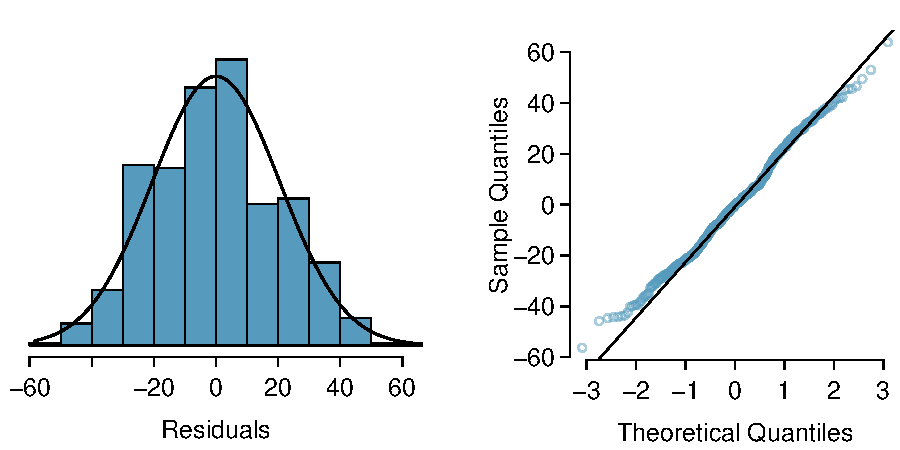
\includegraphics[width=0.8\textwidth]
	{ch_multiple_linear_regression_oi_biostat/figures/RFFTStatinAgeEducCVDResidNormPlot/RFFTStatinAgeEducCVDResidNormPlot.pdf}
	\caption{A histogram and normal probability plot of the residuals from the linear model for RFFT vs. statin use, age, educational level and presence of cardiovascular disease in the PREVEND data}
	\label{RFFTStatinAgeEducCVDResidNormPlot}
\end{figure}

It is quite possible that even the model summarized in
Table~\ref{RFFTStatinAgeEducationCVD} is not the best one to understand
the association of cognitive ability with statin use.  There may well be
other confounders not accounted for.  Possible predictors that may be
confounders but have not been examined are called \term{residual
confounders}.  Residual confounders can be other variables in a dataset
that have not been examined, or variables that were not measured in the
study.  Residual confounders exist in almost all observational studies,
and is one of the main reasons that observational studies should be
interpreted with caution.  A randomized experiment is the best way to
eliminate residual confounders, since randomization insures that, at
least on average, all predictors are not associated with the randomized
intervention, eliminating one of the conditions for confounding.  A
randomized trial may be possible in some settings; there have been many
randomized trials examining the effect of using statins. But in many
other settings, such as a study of the association of marijuana use and
later addiction to controlled substances, randomization may not be
possible or ethical.  In those instances, observational studies may be
the best available approach. They should be analyzed carefully and
thoughtfully.

\section{Interaction in regression}

Use NHANES

\section{Model selection and prediction}

Forest birds

\section{The connection between ANOVA and regression}

Statins and education, refer to ch 5


\section{Notes}

This and the previous chapters have provided only an introduction to regression, with many advance topics not covered. But even this introduction provides useful tools for getting started on many analyses by following some commonly recommended steps.

\begin{itemize}
	
	\item Regression models are more reliable when the response variable has an approximate normal distribution, or at least a symmetric distribution.  Always begin by examining a histogram and normal probability plot of the response variable.  Right-skewed response variables are common, and a log transform will often produce approximate normality. The predictors need not be normally distributed; some may be categorical variables.  If a transformation is used for the response variable, the final interpretation of the any model should be stated in terms of the original scale of measurement for the response.
	
	\item When fitting a simple linear regression, make a scatterplot with a least squares line, even when the predictor is a categorical variable with two levels.  Nonlinear trends or outliers are often obvious in scatterplots.  If outliers are evident, the source of the data should when possible, since outliers result from errors in data collection.  If there has not been an error or the data collection process is not accessible, consider whether the outlier does not belong to the target population of inference, such as the District of Columbia in the data on infant mortality shown in Figure~\ref{infMortUS}.
	
	\item Keep a clear view of the purpose of the regression.  Will it be used to understand the relationship between a particular predictor and the response after adjusting for confounders, to construct a model for prediction, or to simply understand the joint association between a response and set of predictors.
	
	\item Building a model for prediction from a large set of potential predictors can be useful, but the best way to construct a multiple regression model is to think about the context of the problem and include predictors that have either been shown in the past to be associated with the response or for which there is a plausible working hypothesis about some association.
	
	\item When building a model where there may not be a clear specification of which predictors to include, it is useful to examine the association between the response and each of the individual predictors.  Remember that lack of statistical significance of the association between a response and a predictor is not evidence of no association, so predictors are often included in an initial model even when the evidence against no association is weaker than the traditional $p=0.05$.  In practice, investigators sometimes include predictors for which the individual associations are significant at $p < 0.10$ or $p < 0.20$.
	
	\item  With either simple or multiple regression, examine diagnostic plots of the residuals before drawing conclusions.  All models are approximations, and residual plots are seldom as perfectly behaved as in \data{statin.samp}, so don't fuss too much about relatively minor violations of the assumptions.  When the residual plots show some striking anomalies, as in the analysis of the \data{famuss} dataset, try to explore the anomalies for an explanation.  Even when they can't be `disappeared', it is useful to understand the source of the anomalies.
	
	\item  The summary statistics from a regression output, e.g., t-statistics, adjusted $R^2$ and $F$-statistics all provide different information and should be used appropriately.


  \begin{comment}
    multivariate definition of R-squared
  \end{comment}
\end{itemize}

To keep the treatment of regression both brief and accessible, however, many important topics have been left out.  Here are some of the most important

\begin{itemize}
	
	\item Predicted values from a regression have an inherent uncertainty because model parameters are only estimates.  There are two types of interval estimates used with prediction: confidence intervals for a predicted mean response from a set of values for the predictors; and prediction intervals that show the variability in predicted response for a set of predictors for a case not in the dataset.  Because prediction intervals are subject to both the variability in a predicted mean response and the variability of an individual observation about is mean, prediction intervals are wider than confidence intervals for a predicted mean.  Most statistical software provide both kinds of estimates.
	
	\item Model selection is a more advanced and more difficult topic that is often recognized by practitioners, and about which there is continuing research.  Many introductor texts recommend using `stepwise' regression.  Forward stepwise regression adds predictors one by one according to a set criterion (usually smallest $p$-value).  Backward stepwise regression eliminates variables from a larger model one by one until a criterion is met. Both approaches can be useful and usually automated in statistical software.  But there are weaknesses to both methods -- final models are data dependent and chance alone can lead to spurious variables being included.  Since the models are data-driven, traditional formulas for estimating prediction error underestimate the variability in predictions. In very large datasets, stepwise regression can lead to substantially incorrect models. Newer methods for model building based on cross-validation or other advanced techniques are more reliable.
	
	\item  Examining the significance levels of several regression coefficients involves (at least implicitly) testing several hypotheses simultaneously and can lead to increased type I error rate, of the sort discussed in Section~\ref{multipleComparisonsAndControllingTheType1ErrorRate}.  A less error-prone approach begins with the $F$statistic, and if it significant, adjusts $p$-value for multiplicity. For a small number of coefficients, a Bonferroni adjustment is useful, but more advanced methods of error control are used in datasets with more than a handful of parameters.  \textit{we are not following our own advice on this.}
	
\end{itemize}


 
\begin{comment}

  - Add an data exercise showing that r-squared always increases but
  that the adjusted r-squared 

  - the section that introduces general multiple regression mentions
  several applications of multiple regression (model selection, ANOVA)
  but never illustrates those apps.  We should have a section on model
  selection.  What about interaction in regression.

\end{comment}




 
 
